% David
\section{Gefahrengüter}
\subsection{Was sind Gefahrengüter – und warum sind sie relevant?}

Gefahrengüter sind Stoffe und Gegenstände, die beim Transport eine
Gefahr für Menschen, Umwelt oder Sachwerte darstellen. Sie werden nach
internationalen Regelwerken in neun Hauptklassen und diverse Unterklassen
eingeordnet. Für jede Klasse gelten spezifische Kennzeichnungspflichten,
Verpackungsvorschriften und Dokumentationsanforderungen.

\begin{center}
  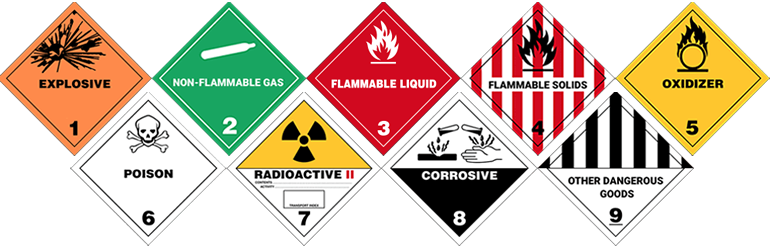
\includegraphics[width=0.7\linewidth]{./assets/gg-dangerous-shields.png}
\end{center}

Für die Beförderung existieren je nach Transportweg unterschiedliche Vorschriften:
\textbf{ADR} (Straße), \textbf{IMDG} (See), \textbf{RID} (Schiene) und \textbf{IATA} (Luft).
Diese Regelwerke definieren unter anderem zulässige Mengen, Verpackungsarten und
Begleitdokumente.

\subsection{Relevanz im ERP‐System}
\begin{itemize}
  \item Korrekte \textbf{UN-Nummer} und \textbf{Gefahrgutklasse} sind für
        Versand, Lagerung und Zollabwicklung zwingend.
  \item Fehlende oder falsche Klassifizierung führt zu
        Verzögerungen, Bußgeldern oder Transportrisiken.
  \item Automatisierte Plausibilitätsprüfungen verringern manuellen
        Aufwand und Fehlerquoten in den Stammdaten.
\end{itemize}